\documentclass[serif,mathserif,final]{beamer}

\mode<presentation>{\usetheme{Lankton}}

\setbeamertemplate{caption}[numbered] % number figs
\usepackage[
  orientation=landscape,
  %size=custom,width=121.92,height=91.44,%
  size=a0, % paper size
  scale=1.1 % font scale factor
]{beamerposter}

% Packages without options
\usepackage{
  amsmath,amssymb, % math
	siunitx, % units
	cleveref,% cross-references
	physics, % better physics notation
	url, % for URLs
	amsmath, % for math
	nth, % for \nth{90}
  xspace, % for spacing
  graphicx, % for pictures
  mdframed,
}
\newcolumntype{L}[1]{>{\raggedright\let\newline\\\arraybackslash\hspace{0pt}}m{#1}}
\graphicspath{{../../figures/}{./}}

\sisetup{round-mode = figures, round-precision = 3}

% MACROS
\newcommand*{\eg}{e.g.\@\xspace}
\newcommand*{\ie}{i.e.\@\xspace}

% this package loads last except for biblatex
\usepackage{cleveref}

\usepackage[
	backend=biber,
	url=false,
	isbn=false,
	style=numeric-comp,
	uniquename=false,
	uniquelist=false,
	firstinits=true,
	sorting=none,
	natbib=false,
	isbn=false,
]{biblatex}

\renewbibmacro{in:}{}

\renewcommand*{\bibfont}{\footnotesize}

\ExecuteBibliographyOptions{
	doi=false,
	maxnames = 2,
}

% One-paragraph bibliography environment
\defbibenvironment{bibliography}
	{\list%
		{\printtext[labelnumberwidth]{%
			\printfield{prefixnumber}%
			\printfield{labelnumber}}%
		\ifentrytype{article}{}{}}%
			{\setlength{\leftmargin}{0pt}%
			\setlength{\topsep}{0pt}}%
			\renewcommand*{\makelabel}[1]{##1}}%
		{\endlist}%
{\mkbibitem}

% \mkbibitem just prints item label and non-breakable space
\makeatletter
	\newcommand{\mkbibitem}{\@itemlabel\addnbspace}
\makeatother

% Add breakable space between bibliography items
\renewcommand*{\finentrypunct}{\addperiod\space}

\AtEveryBibitem{%
	\clearfield{month}%
	\clearfield{day}%
  \clearlist {language}%why this has to be clear list.....
  \clearfield{pages}%
	\clearfield{pagetotal}%
	\clearfield{eprinttype}%
	\clearfield{eprint}%
	\clearfield{number}%
	\clearfield{volume}%
	\clearfield{issue}%
	\clearfield{name:given}
	\clearfield{name:first}
	\ifentrytype{article}{
    \clearfield{title}%
	}%
}
\setbeamertemplate{bibliography item}[text] % don't print the silly symbols

\addbibresource{../library.bib}

%-- Header and footer information ----------------------------------
\newcommand{\footleft}{DOI: \url{10.13140/RG.2.2.20146.30406}}
\newcommand{\footright}{Corresponding author: \url{james.doss-gollin@columbia.edu}}
\title{A31H-2289: Causes and Model Skill of the Persistent Intense Rainfall and Flooding in Paraguay during the Austral Summer 2015-2016}
\author{James Doss-Gollin\inst{1} \quad \'{A}ngel G. Mu\~{n}oz\inst{2} \quad Simon J. Mason\inst{3} \quad Max Past\'{e}n\inst{4}}
\institute{
  \inst{1} Columbia Water Center, Columbia University \quad
  \inst{2} AOS, Princeton University \quad
  \inst{3} International Research Institute for Climate and Society, Columbia University \quad
  \inst{4} Direcci\'{o}n de Meteorolog\'{i}a e Hidrolog\'{i}a, Paraguay
}

%-- Main Document --------------------------------------------------

%-- Main Document --------------------------------------------------
\begin{document}
\begin{frame}{}
  \begin{columns}[t]

    %-- Column 1 ---------------------------------------------------
    \begin{column}{0.23\linewidth}

      \begin{block}{At a Glance}
  Beginning in Nov. 2015, repeated intense rainfall events associated with mesoscale convective activity caused severe flooding along the Paraguay-Paran\'{a} river system (\cref{fig:study-area}, red box), \emph{displacing over 170000 people}.
  We use a weather typing approch within a diagnostic approach to show that:
  \begin{itemize}
    \item Moisture and energy advection via the South American Low-Level Jet \cite{Marengo:2012cm}, particularly during ``No-Chaco'' events \cite{Vera:2006ib} favored mesoscale convective activity
    \item Strong El Ni\~{n}o favored strong SALLJ but MJO and Atlantic dipole pattern contributed to jet exit region (thus No-Chaco SALLJ events)
    \item Raw S2S model forecasts of rainfall had limited skill beyond 10-15 days, but statistical methods -- particularly the PCR and CCA methods that correct both spatial patterns and magnitudes -- substantially improve forecast skill
  \end{itemize}
  \begin{mdframed}
  \begin{figure}
  	\noindent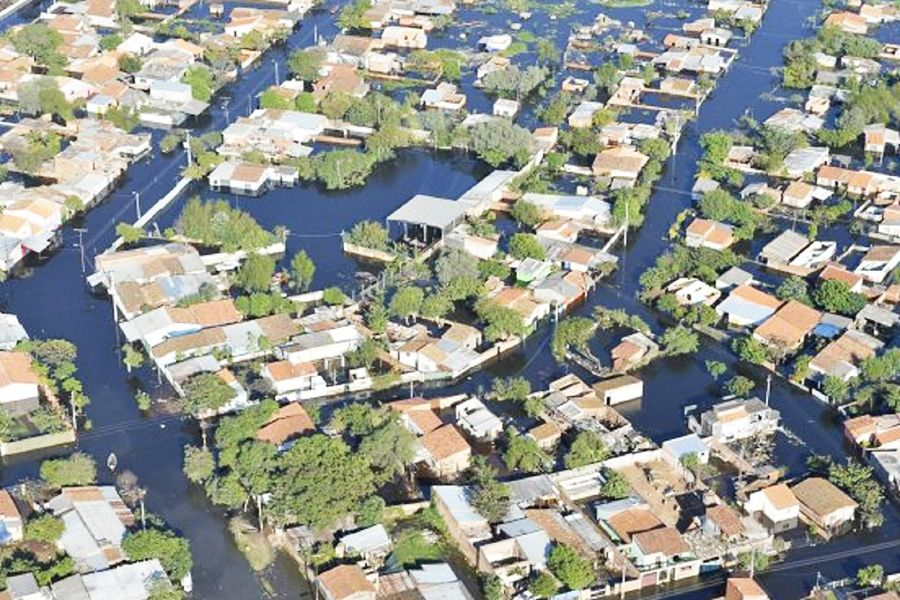
\includegraphics[width=0.45\textwidth]{asuncion-inundaciones.jpg}~
    \noindent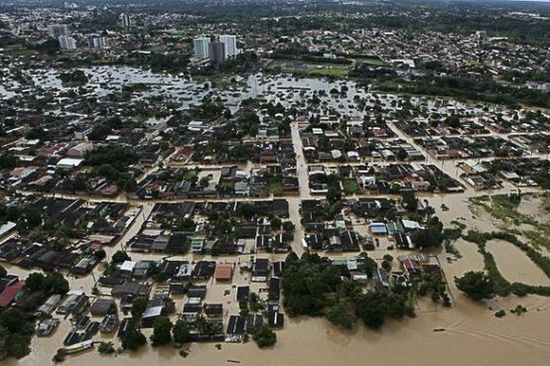
\includegraphics[width=0.45\textwidth]{rio-py-banados.jpg}
  	\caption{
  		Asuncion, Paraguay, 2015-16
  	}
    \label{fig:floods}
  \end{figure}
  \end{mdframed}
\end{block}

      \begin{block}{Observations and Weather Types}
  Observations come from:
  \begin{itemize}
    \item Rainfall: CPC Global Unified \cite{xie2010cpc}
    \item Atmosphere: NCAR-NCEP Reanalysis II \cite{Kanamitsu:2002kk}
  \end{itemize}
  We use weather typing \cite{Munoz2015} to represent daily circulation patterns:
  \begin{enumerate}
    \item Calculate streamfunction $\Psi$ from meridional and zonal wind \cite{Dawson:2016ge}
    \item Project \SI{850}{\hecto\pascal} streamfunction onto leading 4 EOFs
    \item $K$-means clustering using classifiability index \cite{Michelangeli1995} to generate single weather type for each day
  \end{enumerate}
  Weather typing simplifies dynamics of daily rainfall but \emph{facilitates analysis of sequences of daily weather patterns}.
  They are associated with patterns that have been well described in the literature; particularly relevant are:
  \begin{itemize}
    \item WT1 represents ``Chaco'' jet event \cite{Salio:2002ev}
    \item WT4 represnts ``No-Chaco'' jet events \cite{Vera:2006ib}
  \end{itemize}
  \begin{mdframed}
  \begin{figure}
  	\noindent\includegraphics[width=0.925\textwidth]{weather-type-composite-alt.pdf}
  	\caption{
  		Colors: anomalies of rainfall associated with each weather type [\si{\milli\meter\per\day}].
      Contours: anomalies of \SI{850}{\hecto\pascal} streamfunction [contour interval \SI{1e4}{\meter\squared\per\second}]
  	}
    \label{fig:weather-types}
  \end{figure}
  \end{mdframed}
% \item S2S forecasts issued by ECMWF \cite{Vitart2016}
\end{block}


    \end{column}%1

    %-- Column 2 ---------------------------------------------------
    \begin{column}{0.23\linewidth}

      \begin{block}{Observed Circulation Anomalies}
  \begin{mdframed}
  \begin{figure}
    \caption{
  		Daily rainfall averaged over Lower Paraguay River Basin and observed weather type for each day in NDJF 2015-16.
      Blue lines indicate the climatological 50th, \nth{90}, and 99th percentiles of NDJF area-averaged rain.
      \label{fig:rain-wt}
  	}
    \noindent\includegraphics[width=0.925\textwidth]{wt-rain-time-series.pdf}
    \end{figure}
  \end{mdframed}

  During austral summer (NDJF) 2015-16, most heavy rainfall occurred during weather types 1 and 4 (\cref{fig:rain-wt}).
  Monthly-scale circulation anomalies (\cref{fig:anomalies}) show a weak anticyclonic circulation that set up over central Brazil during November 2015 and strengthened into the following month.
  In January 2016 it weakened before returning in February 2016.
  The observed rainfall and circulation anomalies are consistent with the aggregation of the observed weather types shown in \cref{fig:rain-wt}.

  \begin{mdframed}
  \begin{figure}
  	\noindent\includegraphics[width=0.925\textwidth]{circulation-NDJF-1516-anomaly-alt.pdf}
  	\caption{
      	Monthly composite anomalies observed during NDJF 2015-16.
        Colors: anomalies of rainfall associated with each weather type [\si{\milli\meter\per\day}].
        Contours: anomalies of \SI{850}{\hecto\pascal} streamfunction [contour interval \SI{1e4}{\meter\squared\per\second}]
        \label{fig:anomalies}
  	}
  \end{figure}
  \end{mdframed}
\end{block}

      \begin{block}{Lower Paraguay River Basin}
  Flat topography limits the river's ability to carry the summer runoff, causing seasonal inundation of the Pantanal and distributing the river discharge in time \cite{Bravo:2011et,Barros:2004bn}.
  During NDJF 2015-16, river stage [height] throughout the Lower Paraguay River Basin reached nearly three times climatological levels (not shown).
  \begin{mdframed}
  \begin{figure}
  	\noindent\includegraphics[width=0.8\textwidth]{study-area.jpg}
  	\caption{
  		Topographical map of the study area.
  	}
    \label{fig:study-area}
  \end{figure}
  \end{mdframed}
\end{block}

      \begin{block}{Acknowledgements}
  This research was supported by funding from NSF Sustainability Research Networks (award 1444745): ``Integrated Urban Infrastructure Solutions for Environmentally Sustainable, Healthy, and Livable Cities'' and  SERDP grant \#2516: ``Climate Informed Estimation of Hydrologic Extremes for Robust Adaptation to Non-Stationary Climate''.
  The authors thank Yochanan Kushnir and James Booth for conversations regarding this work, and Casey Brown, Melissa Bukovsky, Rachel McCrary, Seth McGinnis, Linea Mearns, and Katherine Schlef for collaboration and advice.
\end{block}


    \end{column}%2

    %-- Column 3 ---------------------------------------------------
    \begin{column}{0.23\linewidth}

      \begin{block}{S2S  Model Forecasts}
  \begin{mdframed}
  \begin{figure}
    \caption{
      Chiclet diagram of ensemble-mean precipitation anomaly forecasts over the Lower Paraguay River Basin from ECMWF S2S forecast data, as a function of the forecast target date (horizontal axis) and lead time (vertical axis).
      Time series of daily precipitation over the same area is plotted with $y$-axis inverted.
  	}
    \noindent\includegraphics[width=0.925\textwidth]{chiclet-s2s-area-averaged.pdf}
  	\label{fig:chiclet}
  \end{figure}
  \end{mdframed}

  \Cref{fig:chiclet} uses a Chiclet diagram \cite{Carbin:2016fx} to visualize, as a function of lead time, the time evolution of the uncorrected, ensemble-mean rainfall anomaly forecast, spatially averaged over the Lower Paraguay River Basin.
  At lead times greater than about two weeks, the ensemble-mean forecast is slightly wetter than climatology.
  At weather timescales (less than one week), the ensemble-mean successfully predicts the timing and amplitude of the area-averaged rainfall.
  At intermediate timescales, the model successfully forecast the strongest breaks and pauses in the rainfall, such as the heavy rainfall during December 2015 and the dry period during mid-January 2016.

  \end{block}
  \begin{block}{Model Output Statistics}

  We explore whether using Model Output Statistics \cite[MOS;][]{Glahn:1972vt} can improve the modeled representation of rainfall (\cref{fig:subs-prob-fcst}).
  Specifically, we use: the raw model output (Raw); extended logistic regression \cite[XLR;][]{Wilks:2009bk}; heteroscedastic XLR \cite[HXLR;][]{Messner:2014gp}; principal component regression \cite[PCR;][]{Mason:2008da,Wilks:2006fx}; and canonical correlation analysis \cite[CCA;][]{Mason:2008da,Barnston:1992gd} using 20 years of ECMWF forecasts.

  \vspace{0.5cm}

  \Cref{fig:subs-prob-fcst} indicates that better forecasts are obtained when both magnitude and spatial corrections are performed (PCR and CCA).
  The enhanced skill is achieved through the spatial corrections via the EOF-based regressions, which -- in contrast with the extended logistic models -- use information from multiple grid-boxes,.

  \begin{mdframed}
  \begin{figure}
  	\noindent\includegraphics[width=0.925\textwidth]{s2s-forecast-mos.pdf}
  	\caption{
    MOS-adjusted S2S model forecasts and skill scores.
    Top row shows the heavy rainfall ($>$\nth{90} percentile exceedance) forecast for 1-7 December 2015 as the odds ratio $\text{odds}_{r} \equiv \frac{p}{\qty(1 - p)} \frac{\qty(1 - p_c)}{p_c}$.
    Second row shows the Ignorance score $\text{IGN} \equiv - \log_2 p(Y)$.
    Bottom row shows the 2AFC skill score for each grid cell.
    For all three rows, the grid cells which experienced a \nth{90} percentile exceedance for 1-7 December 2015 are outlined in black.
        \label{fig:subs-prob-fcst}
  	}
  \end{figure}
  \end{mdframed}
\end{block}


    \end{column}%3

    %-- Column 4 ---------------------------------------------------
    \begin{column}{0.23\linewidth}

      \begin{block}{S2S Drivers of Weather Patterns}
  \begin{mdframed}
  \begin{figure}
    \caption{
  		Anomalous probability of occurrence of each weather type concurrent with observance of each MJO and ENSO phase.
  		Only values which are significant at $p<0.10$ are shown.
      \label{fig:wt-mjo-enso}
  	}
  	\noindent\includegraphics[width=0.925\textwidth]{wt-mjo-enso.pdf}
  \end{figure}
  \end{mdframed}

  During El Ni\~{n}o years such as 2015-16, weather type 1 -- related to Chaco jet events -- occurs more frequently for almost all MJO phases, and particularly during phases 1, 2, and 5, consistent with observations of the year under study.
  This agreesß with previous studies \cite[i.e.][]{Velasco1987} which find that the intensity and exact location of the anomalous low-level anticylonic anomaly over central Brazil is relevant for the precise impact of ENSO events.

  \vspace{0.5cm}

  While the occurrence of WT1 during NDJF 2015-16 is well explained by ENSO and MJO variability, these features alone do not explain the occurrence of WT4, the ``No-Chaco'' jet event.
  Previous studies emphasize the importance of Pacific-Atlantic interaction for forecasting climate effects in this region \cite{Vera:2006ib,Barreiro:2017ct,Lima:2017hw,Munoz2015}.
  A persistent SST dipole in the central southern Atlantic Ocean favors the occurrence of WT4 by blocking transient extratropical wave activity coming from the Pacific, facilitating transitions from Chaco jet events (WT 1) to No-Chaco jet events (WT 4) via enhanced low-level wind circulation from southern Brazil towards the Atlantic, and back to north-east Brazil and the Amazon (see \cref{fig:chaco-nochaco}) due to land-sea temperature contrasts.

  \vspace{0.5cm}

  Composite analysis (not shown) of months with many WT4 occurrences is consistent with the schematic shown here.

  \begin{mdframed}
  \begin{figure}
  	\noindent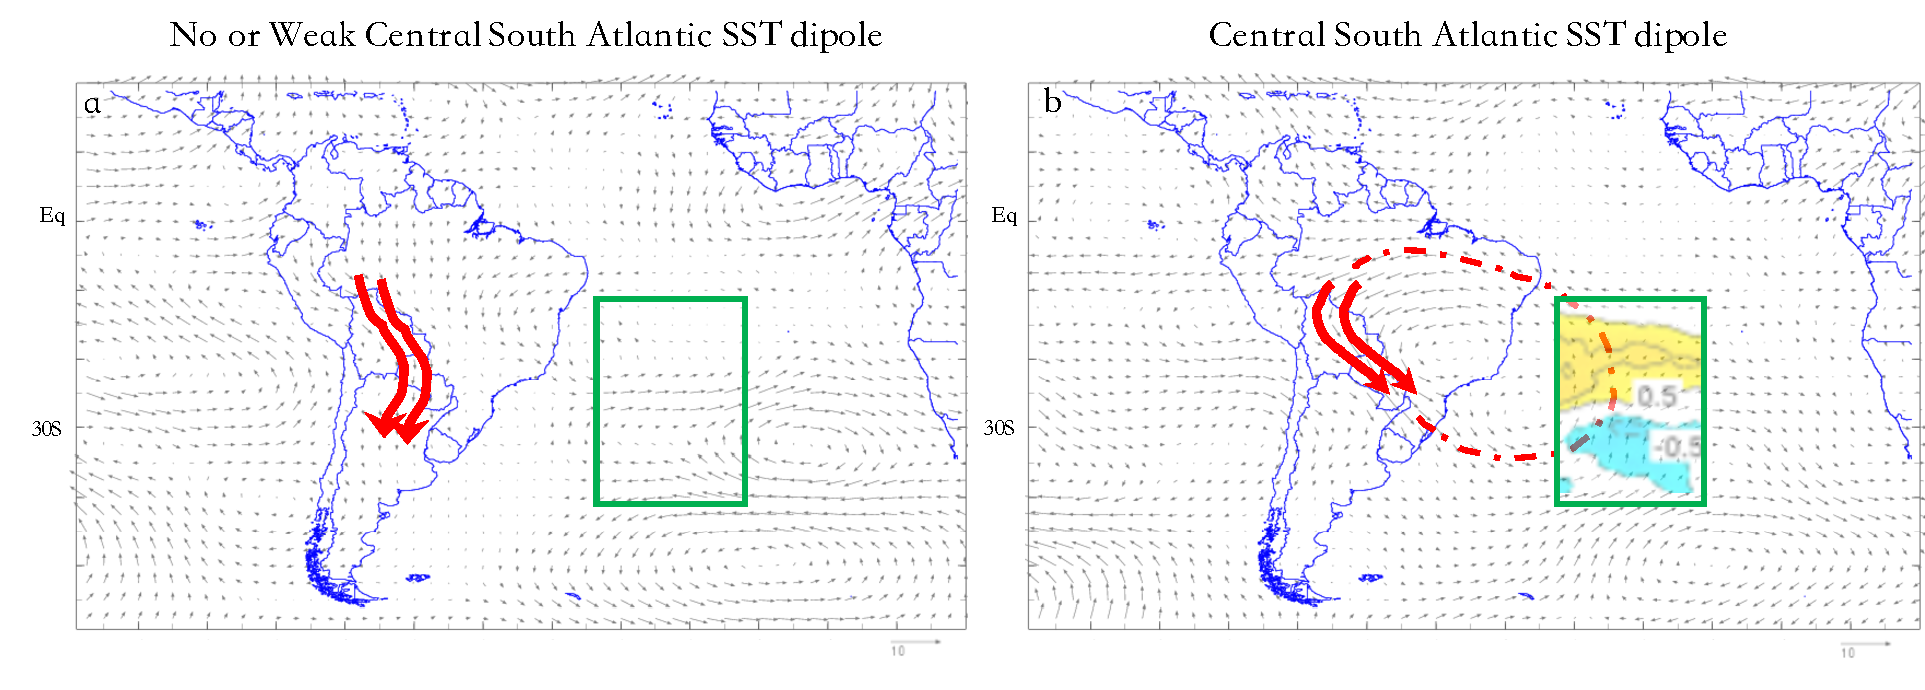
\includegraphics[width=0.925\textwidth]{../writeup/ChacoNoChacojet.pdf}
    \caption{
      Simple schematics of low-level jet events (red arrows) during austral summer and El Ni\~no years.
      \label{fig:chaco-nochaco}
  	}

  \end{figure}
  \end{mdframed}
\end{block}

      \vfill
      \begin{block}{References}
  \printbibliography[heading=none]
\end{block}


    \end{column}%1

  \end{columns}
\end{frame}
\end{document}
